\documentclass[conference]{IEEEtran}
\IEEEoverridecommandlockouts
\usepackage{cite}
\usepackage{amsmath}
\usepackage{newtxtext,newtxmath} % Times, as IEEE requires
\usepackage{graphicx}
\usepackage{booktabs}
\usepackage{multirow}
\usepackage{siunitx}
\usepackage{xcolor}
\usepackage[hidelinks]{hyperref}
\sisetup{detect-all}
\graphicspath{{figures/}}
\newcommand{\cotwo}{CO$_2$}

\begin{document}

\title{Faster Is Not Greener: A Meter-Calibrated Study of\\
Carbon-Aware Client Selection in Heterogeneous Federated Learning}

% Double-blind submission: keep the author block anonymous.
\author{\IEEEauthorblockN{Anonymous Author(s)}
\IEEEauthorblockA{Submission to IEEE CCGrid 2027, Sustainable Computing and Green Technologies track}}

\maketitle

\begin{abstract}
Federated learning (FL) deployments increasingly run on heterogeneous commodity machines whose speed and power draw differ widely. Client-selection policies typically favour fast participants, implicitly assuming that faster hardware is also more efficient. We test that assumption with wall-meter measurements and use the measurements to calibrate a carbon-aware client-selection study. On an identical CPU-only CIFAR-10 FedAvg workload (50 clients, 10 per round, Dirichlet $\alpha{=}0.1$, 3000 rounds), a 265K-class desktop finished 28.4\% sooner than a 235-class desktop but drew 2.43$\times$ the average power and consumed 73.9\% more energy, with the same accuracy within run-to-run noise. We then build a simulator that trains a real FedAvg model while modelling round time, energy (including idle participants and the coordinator) and grid emissions from the measured node profiles, and we train a tabular multi-objective Q-learning selector whose state and reward use only validation data. Across five paired data seeds, the learned selector reduces modelled emissions by 43.7\% (95\% CI of the paired difference: $-8.21$ to $-7.70$\,g over 20 rounds) and round time by 8.4\% relative to selecting all clients, at a cost of 1.35 accuracy points (95\% CI: $-2.16$ to $-0.53$). Simple fixed rules remain competitive: selecting the two lowest-energy clients emits 38\% less than the learned selector at statistically indistinguishable accuracy. We release the measurement records, simulator and evaluation protocol, and we discuss when learned selection is, and is not, worth its complexity.
\end{abstract}

\begin{IEEEkeywords}
federated learning, client selection, carbon-aware computing, energy measurement, reinforcement learning, heterogeneous systems
\end{IEEEkeywords}

\section{Introduction}

Federated learning (FL) trains a shared model across many participants that keep their data local~\cite{mcmahan2017fedavg,kairouz2021advances}. In practice, the participants of a cross-silo or on-premise deployment are often whatever machines are available: desktops of different generations, with different CPUs, memory and accelerators. Because a synchronous FedAvg round ends only when the slowest selected participant reports, most client-selection work optimises time-to-accuracy and favours fast participants~\cite{nishio2019client,lai2021oort}.

The energy and carbon cost of training is now a first-class concern~\cite{strubell2019energy,henderson2020systematic,lacoste2019quantifying}, and FL is no exception~\cite{qiu2023carbon}. A selection policy that prefers the fastest machines makes an implicit assumption: that the time saved is not paid back in energy. Modern desktop processors break this assumption easily. Higher-tier parts reach their speed by drawing far more power, so the energy per unit of work can rise even as latency falls.

This paper makes that trade-off concrete and asks whether a learned selector can navigate it. Our contributions are:

\begin{enumerate}
\item \textbf{A wall-meter measurement} of two contemporary desktops running an identical CPU-only CIFAR-10 FedAvg workload. The faster machine finished 28.4\% sooner but consumed 73.9\% more energy (Section~\ref{sec:measure}).
\item \textbf{A meter-calibrated FL simulator} that trains a real model with FedAvg and attributes time, energy and emissions to every node in every round, including idle participants and the coordinator. Every reported quantity carries an explicit provenance label: measured, computed from measurement, or assumed (Section~\ref{sec:system}).
\item \textbf{A carbon-aware tabular multi-objective Q-learning selector} evaluated under a leakage-free, paired protocol: the agent observes only validation accuracy, every repeat regenerates its data, and all policies share each repeat's data and timing noise (Sections~\ref{sec:rl}--\ref{sec:method}).
\item \textbf{An honest comparison.} The learned selector reduces emissions by 43.7\% and time by 8.4\% relative to all-client FedAvg at a 1.35-point accuracy cost, but a fixed lowest-energy rule emits even less. We analyse why, and identify the conditions under which learned selection should pay off (Sections~\ref{sec:results}--\ref{sec:discussion}).
\end{enumerate}

\section{Related Work}

\textbf{Client selection.} FedCS~\cite{nishio2019client} selects participants that can finish within a deadline on heterogeneous mobile-edge resources. Oort~\cite{lai2021oort} ranks participants by a combination of statistical utility and system speed to reduce time-to-accuracy. FAVOR~\cite{wang2020favor} uses deep Q-learning to choose participants that counter non-IID bias. These methods target accuracy and time; energy and emissions are not part of their objective.

\textbf{Energy- and carbon-aware FL.} Yang et al.~\cite{yang2021energy} jointly optimise computation and transmission energy for FL over wireless links. Qiu et al.~\cite{qiu2023carbon} provide a first systematic estimate of FL's carbon footprint and compare it with centralised training. FedZero~\cite{wiesner2024fedzero} schedules participants onto renewable excess energy and spare capacity. Carbon-aware scheduling in datacentres shifts flexible load in time and space according to grid intensity~\cite{radovanovic2023carbon}. Our work is complementary: we focus on the \emph{hardware} side of the trade-off, measure it with a physical meter, and study selection among participants that share one grid.

\textbf{Measurement and reporting.} Henderson et al.~\cite{henderson2020systematic} and Lacoste et al.~\cite{lacoste2019quantifying} argue for systematic, transparent reporting of the energy and carbon cost of ML. Software estimators are convenient, but they do not observe whole-system draw. We report physical wall-meter readings and label every derived or assumed quantity, so readers can separate evidence from modelling.

\textbf{Multi-objective RL.} Scalarising a vector reward with fixed weights is the simplest multi-objective RL approach~\cite{hayes2022morl}. We use it deliberately: with few clients the action space is small enough for a tabular agent~\cite{watkins1992qlearning}, which keeps the learned policy fully inspectable.

\section{Measurement Study: Faster Is Not Greener}\label{sec:measure}

\subsection{Setup}

We ran the same FL training job on two desktops, PC2 (Intel Core Ultra~5~235, 16\,GB RAM, integrated graphics) and PC3 (Intel Core Ultra~7~265K, 32\,GB RAM, 8\,GB discrete GPU with CUDA disabled). The job simulates FedAvg on CIFAR-10~\cite{krizhevsky2009cifar} with 50 clients, 10 sampled per round, a Dirichlet label partition with $\alpha{=}0.1$~\cite{hsu2019noniid}, and 3000 rounds, executed entirely on the CPU. Each machine was connected through an external physical electricity meter with \SI{0.001}{kWh} resolution; we recorded the meter reading at the start and end of each run together with the elapsed time. Emissions are computed as measured energy multiplied by the Indian grid's FY~2025--26 weighted-average emission factor, \SI{0.675}{kg\,CO_2/kWh}~\cite{cea2026baseline}.

\subsection{Results}

Table~\ref{tab:measured} and Fig.~\ref{fig:measured} summarise the two runs. PC3 completed the job in 137.5 minutes against PC2's 192.1 minutes, a 28.4\% reduction in wall time (39.7\% higher throughput). Its average draw, however, was 209.4\,W against 86.2\,W, so it consumed 0.480\,kWh against 0.276\,kWh: 73.9\% more energy, and therefore 73.9\% more emissions under a fixed grid factor. Per round, PC3 used \SI{0.160}{Wh} against \SI{0.092}{Wh}. Final accuracy differed by 0.35 points (72.46\% vs 72.11\%). The workload and configuration were identical, so this gap reflects run-to-run nondeterminism rather than any effect of the hardware.

\begin{table}[t]
\centering
\caption{Wall-meter measurements, identical CPU-only CIFAR-10 FedAvg job (3000 rounds). PC2: Core Ultra 5 235; PC3: Core Ultra 7 265K.}
\label{tab:measured}
\begin{tabular}{@{}lrr@{}}
\toprule
 & PC2 & PC3 \\
\midrule
Wall time (min) & 192.1 & 137.5 \\
Energy, meter delta (kWh) & 0.276 & 0.480 \\
Average power (W) & 86.2 & 209.4 \\
Time per round (s) & 3.84 & 2.75 \\
Energy per round (Wh) & 0.092 & 0.160 \\
Emissions at 0.675 kg/kWh (g) & 186.3 & 324.0 \\
Final test accuracy (\%) & 72.11 & 72.46 \\
\bottomrule
\end{tabular}
\end{table}

\begin{figure}[t]
\centering
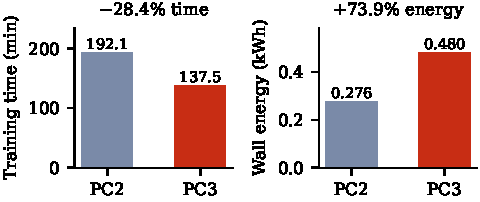
\includegraphics[width=\columnwidth]{measured_benchmark.pdf}
\caption{Measured wall time and wall energy for the same job on PC2 (Core Ultra 5 235) and PC3 (Core Ultra 7 265K). The faster machine uses substantially more energy.}
\label{fig:measured}
\end{figure}

\subsection{Implication for selection}

The ratio of power to speed decides which machine is greener for a fixed amount of work. Here PC3 is 1.40$\times$ faster but draws 2.43$\times$ the power, so each unit of work costs 1.74$\times$ the energy. A speed-first policy would choose PC3 every round and pay that premium on every round. A synchronous round also forces faster selected participants to wait for the slowest, so the latency gain from a fast machine is realised only when every other selected machine is also fast. Selection should therefore weigh speed, power and the composition of the selected set together. This motivates the remainder of the paper.

\section{Meter-Calibrated FL Simulator}\label{sec:system}

Measuring every candidate policy on physical hardware for many repeats is expensive, so we evaluate selection policies in a simulator whose node profiles come from the measurements above, while the learning itself is real.

\subsection{Federated training}

Four virtual clients, PC1--PC4, each hold 250 training samples of a three-class, two-feature classification problem. Class centres are fixed and features carry Gaussian noise ($\sigma{=}1.3$). Labels are non-IID: PC1--PC3 each draw 80\% of their samples from one distinct class, and PC4 is roughly balanced. A separate 500-sample validation set and 1500-sample test set are drawn from the same generator. Each selected client runs two local epochs of gradient descent (learning rate 0.23) on a multinomial logistic-regression (softmax) model, and the server aggregates with sample-weighted FedAvg~\cite{mcmahan2017fedavg}. Accuracy is therefore computed from actual training, not modelled.

\subsection{Node profiles}

Table~\ref{tab:profiles} lists the node profiles. The active power of PC2 and PC3 is the measured average power from Section~\ref{sec:measure}, and their relative speeds preserve the measured ratio (1.54/1.10 = 1.40). PC1's power comes from a single meter reading (0.065\,kWh over 190 minutes) that we flag as unverified, and PC4 is an assumed profile. Idle power, network delay, coordinator power (30\,W) and aggregation time (0.45\,s) are assumptions.

\begin{table}[t]
\centering
\caption{Node profiles used by the simulator, with provenance. $^{\dagger}$Single reading, not yet verified.}
\label{tab:profiles}
\small\setlength{\tabcolsep}{4pt}
\begin{tabular}{@{}lrrrrl@{}}
\toprule
Node & Speed & $P^{\mathrm{act}}$ (W) & $P^{\mathrm{idle}}$ (W) & Net (s) & Source of $P^{\mathrm{act}}$ \\
\midrule
PC1 & 1.00 & 20.5 & 7 & 0.30 & meter$^{\dagger}$ \\
PC2 & 1.10 & 86.2 & 9 & 0.45 & meter \\
PC3 & 1.54 & 209.4 & 13 & 0.60 & meter \\
PC4 & 1.35 & 35.9 & 11 & 0.45 & assumed \\
\bottomrule
\end{tabular}
\end{table}

\subsection{Time, energy and emissions model}

Let $S_r$ be the set of clients selected in round $r$. Client $i$'s training time is $t_i = \tau \xi_{i,r}/s_i$, with base time $\tau{=}16$\,s, relative speed $s_i$, and per-round jitter $\xi_{i,r}\sim\mathcal{U}(0.9,1.1)$. With network delay $n_i$ and aggregation time $a$, the synchronous round time is
\begin{equation}
T_r = \max_{i\in S_r}\left(n_i + t_i\right) + a .
\end{equation}
Every client is powered for the whole round. Selected clients draw active power while training and idle power while waiting; unselected clients idle for the full round. Including the coordinator's power $P_c$, round energy is
\begin{equation}
E_r = \sum_{i} \Big[P_i^{\mathrm{act}} t_i \mathbf{1}[i\in S_r] + P_i^{\mathrm{idle}}\big(T_r - t_i \mathbf{1}[i\in S_r]\big)\Big] + P_c T_r ,
\end{equation}
and emissions are $C_r = E_r \cdot \kappa$ with $\kappa = \SI{0.675}{kg\,CO_2/kWh}$. Counting idle participants matters: a policy that leaves machines switched on but unused does not get their energy for free.

\section{Carbon-Aware Q-Learning Selector}\label{sec:rl}

\textbf{State.} The state combines the training phase (the round index split into four quarters) with the current global model's \emph{validation} accuracy, discretised at 0.50, 0.68, 0.76 and 0.81 into five buckets, for 20 states in total. The test set is never visible to the agent.

\textbf{Actions.} An action selects a subset of two, three or four clients. With four clients there are $\binom{4}{2}+\binom{4}{3}+\binom{4}{4}=11$ actions.

\textbf{Reward.} With validation accuracy $A_r$, the scalarised multi-objective reward is
\begin{equation}
R_r = w_a \Delta A_r - w_t T_r - w_c C_r - w_f \max(0,\, A_{\min} - A_r),
\end{equation}
with $w_a{=}15$, $w_t{=}0.018$\,s$^{-1}$, $w_c{=}0.32$\,g$^{-1}$, $w_f{=}0.6$ and accuracy floor $A_{\min}{=}0.78$.

\textbf{Training.} We use tabular Q-learning~\cite{watkins1992qlearning} with learning rate 0.24, discount 0.86, and $\varepsilon$-greedy exploration decaying linearly from 0.80 to a floor of 0.06 over 130 episodes of 20 rounds. Training episodes cycle over three data sets generated from seeds that are disjoint from the evaluation seeds. At evaluation time the policy acts greedily.

\section{Evaluation Methodology}\label{sec:method}

\textbf{Baselines.} \emph{FedAvg (all 4)} selects every client every round. \emph{Fastest-2} selects the two clients with the lowest estimated round time (PC3 and PC4). \emph{Lowest-energy-2} selects the two clients with the lowest estimated active energy per round (PC1 and PC4).

\textbf{Paired repeats.} We run five repeats. Each repeat regenerates the client, validation and test data from its own seed and draws its own timing jitter. All four policies run on the same data and jitter within a repeat. We report means with 95\% confidence intervals (Student-$t$, $n{=}5$), and paired differences between the learned selector and FedAvg (all 4) with their own intervals.

\textbf{Sensitivity to assumptions.} Because PC2--PC4's profiles are single measurements or assumptions, we draw 70 alternative profile sets. In each, the active power of PC2--PC4 is scaled by a factor from $\mathcal{U}(0.65,1.35)$ and speed by a factor from $\mathcal{U}(0.70,1.30)$, with PC1 as the fixed reference. We report the 5th--95th percentile range of total emissions under these perturbations.

\textbf{Provenance.} Accuracy comes from real training on synthetic data. Round time, energy and emissions are modelled from the profiles in Table~\ref{tab:profiles}. We label them as modelled throughout and never mix them with the measured values of Section~\ref{sec:measure}.

\section{Results}\label{sec:results}

\begin{table*}[t]
\centering
\caption{Policy comparison over 20 rounds, five paired repeats. Accuracy is from real training; time, energy and \cotwo{} are modelled from meter-calibrated profiles. Brackets: 95\% CI; $\pm$: standard deviation. Sensitivity: 5th--95th percentile over 70 perturbed profile sets.}
\label{tab:results}
\begin{tabular}{@{}lccccc@{}}
\toprule
Policy & Final test accuracy (\%) & Total time (s) & Total energy (Wh) & Total \cotwo{} (g) & \cotwo{} sensitivity (g) \\
\midrule
FedAvg (all 4) & 83.92 [83.50, 84.34] & 338.8 $\pm$ 3.2 & 26.96 & 18.20 $\pm$ 0.16 & 15.34--22.33 \\
Fastest-2 & 82.31 [81.11, 83.50] & 254.4 $\pm$ 2.6 & 17.87 & 12.06 $\pm$ 0.15 & 8.70--16.13 \\
Lowest-energy-2 & 82.21 [81.35, 83.08] & 337.2 $\pm$ 3.4 & 9.40 & 6.35 $\pm$ 0.05 & 5.77--7.02 \\
Q-learning (ours) & 82.57 [81.63, 83.51] & 310.3 $\pm$ 4.1 & 15.17 & 10.24 $\pm$ 0.22 & 7.99--12.06 \\
\bottomrule
\end{tabular}
\end{table*}

\begin{figure}[t]
\centering
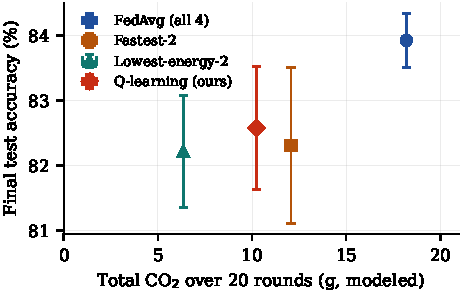
\includegraphics[width=\columnwidth]{accuracy_vs_co2.pdf}
\caption{Final test accuracy against total modelled emissions over 20 rounds (mean of five paired repeats, 95\% CIs). No policy dominates another on all three objectives of accuracy, time and \cotwo{}.}
\label{fig:tradeoff}
\end{figure}

\begin{figure*}[t]
\centering
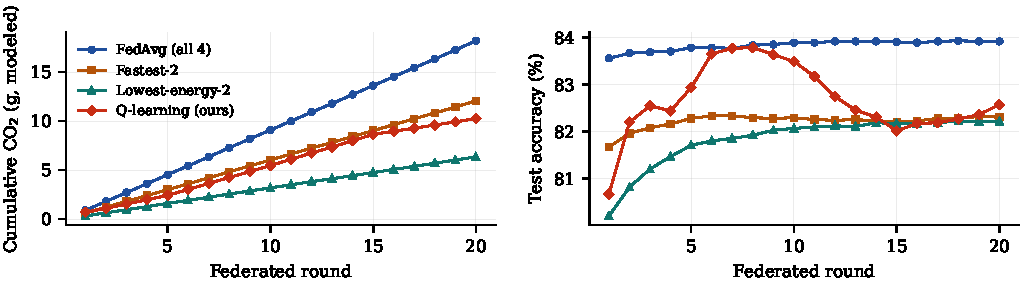
\includegraphics[width=\textwidth]{rounds.pdf}
\caption{Per-round behaviour averaged over five paired repeats. Left: cumulative modelled emissions. Right: test accuracy. The learned selector reaches 83.8\% by round 8 but then drifts down as it shifts to cheaper, more skewed client pairs.}
\label{fig:rounds}
\end{figure*}

\subsection{Learned selection versus all-client FedAvg}

Table~\ref{tab:results} and Fig.~\ref{fig:tradeoff} summarise the comparison. Relative to selecting all four clients, the Q-learning selector reduces total modelled emissions from 18.20\,g to 10.24\,g. The paired difference is $-7.95$\,g (95\% CI $-8.21$ to $-7.70$), or 43.7\%. Total time falls by 28.5\,s (95\% CI $-32.6$ to $-24.3$), or 8.4\%. The cost is accuracy: the paired difference is $-1.35$ points (95\% CI $-2.16$ to $-0.53$), so the loss is small but statistically clear. The emission saving is robust to the profile assumptions. The 95th-percentile emissions of the learned selector under perturbation (12.06\,g) are below the 5th percentile of FedAvg (15.34\,g).

\subsection{What the agent learned}

The selector never chose all four clients. Over 100 evaluation rounds it chose PC1+PC4 in 29\% of rounds, PC1+PC3 and PC3+PC4 in 25\% each, PC2+PC4 in 16\%, and PC1+PC3+PC4 in 5\%. PC4, the assumed low-power and reasonably fast node with balanced labels, participated in 75\% of rounds. The agent therefore learned to keep the balanced client in the federation and to rotate the class-skewed clients around it. That rotation trades a little accuracy for large energy savings.

Fig.~\ref{fig:rounds} shows the cost of that rotation. Mean accuracy peaks at 83.8\% in round 8, level with all-client FedAvg, and then declines to 82.6\%. Once validation accuracy crosses the top bucket edge (0.81), the reward favours cheaper pairs. Pairs that omit one class's majority client bias the global model, and the coarse 20-state representation cannot see that bias. This suggests two improvements: a state that includes per-class or per-client participation information, and a stopping rule that keeps the best validation checkpoint.

\subsection{Fixed rules remain competitive}

Two fixed rules bracket the learned selector. Lowest-energy-2 emits 6.35\,g, 38\% less than the learned selector, at accuracy that is statistically indistinguishable (82.21\% vs 82.57\%, overlapping intervals). Fastest-2 finishes 18\% sooner than the learned selector (254.4\,s vs 310.3\,s) but emits 18\% more, again at similar accuracy. All four policies lie on the three-objective Pareto front of accuracy, time and emissions. No policy is better on all three, and the learned selector sits between the two fixed rules. Its value in this setting is a tunable compromise, not dominance.

The fixed rules also need knowledge that the learned selector does not: which nodes are low-energy or fast. In our setting that knowledge comes directly from the meter. This is the practical lesson of Section~\ref{sec:measure}: once per-node energy is \emph{measured}, a simple energy-ranked rule captures most of the available saving.

\subsection{Accuracy targets}

With an 80\% accuracy target, every policy reaches the target in every repeat. FedAvg (all 4) reaches it in the first round, so time- and energy-to-target comparisons are dominated by the first one or two rounds on this task. We therefore report fixed-horizon totals as our primary metric.

\section{Discussion and Limitations}\label{sec:discussion}

\textbf{When does learned selection pay off?} Under a single, constant grid factor, a node's emissions are a fixed multiple of its energy. The problem then reduces to a static ranking that a fixed rule can exploit. Learned selection should have an advantage when the optimal choice changes over time: grid intensity that varies by hour or by node location~\cite{radovanovic2023carbon,wiesner2024fedzero}, participants whose availability changes, or data heterogeneity that makes \emph{which} clients train together matter for accuracy. Our results isolate the hardware dimension and show that it alone does not require a learned policy.

\textbf{Scale.} With four clients the action space has 11 subsets, small enough for a tabular agent and for exhaustive search. Larger federations need function approximation or ranking-based selection~\cite{lai2021oort,wang2020favor}.

\textbf{Measurement scope.} The meter readings are whole-machine wall energy for one run per machine. We did not record a separate idle baseline, so we cannot split training energy from baseline draw. PC1's reading is a single unverified observation with an unrecorded workload, and PC4 is not measured. The simulated client-selection results use the measured profiles but are not themselves measured on a live multi-machine deployment.

\textbf{Task.} The selection study uses a synthetic three-class problem that saturates within a few rounds. This isolates the systems trade-off, but it understates how much client choice affects accuracy on harder non-IID tasks.

\textbf{Grid factor.} We use the annual weighted-average emission factor. It is neither a marginal nor a real-time intensity, so emissions here scale directly with energy.

\section{Reproducibility}

The measurement records, node profiles, simulator, Q-learning selector, evaluation scripts and the figure-generation script are available at an anonymised repository [link withheld for review]. A full evaluation (130 training episodes, five repeats, 70 sensitivity samples) runs in a few seconds on a laptop CPU. Every output file labels each quantity as measured, computed from measurement, or modelled.

\section{Conclusion}

Faster hardware is not automatically greener. On an identical FL workload, a higher-tier desktop saved 28.4\% of the time but spent 73.9\% more energy. Calibrating an FL simulator with these measurements, a carbon-aware Q-learning selector cut modelled emissions by 43.7\% and time by 8.4\% relative to all-client FedAvg, for a 1.35-point accuracy cost. A fixed lowest-energy rule saved even more emissions at similar accuracy. Two lessons follow for practitioners. First, measure per-node energy before choosing participants, since that measurement alone enables most of the saving. Second, reserve learned selection for settings where the best choice changes over time. Extending the study to time-varying grid intensity, larger federations and live multi-machine measurement is the natural next step.

% IEEE policy requires disclosing any AI-generated content (text, figures, code) in the acknowledgments.
% Complete this before submission; for double-blind review, keep it free of identifying details.
% \section*{Acknowledgment}
% <Disclose AI assistance here, per the IEEE policy on AI-generated content.>

\bibliographystyle{IEEEtran}
\bibliography{refs}

\end{document}
